\section{Méthodologie}

\subsection{Présentation du jeu de données}
Le jeu de données utilisé dans ce travail est composés de différentes statistiques sur les match officiels de l'association des professionnels de tennis (ATP) depuis 1968. Les données sont distribuées par Jeff Sackmann via \textbf{GitHub} et accessible sous ce \href{https://github.com/JeffSackmann/tennis_atp}{lien}.\\

Le jeu de données comprend entres autres la surface sur laquelle un match de tennis a été joué. C'est cette variable que la machine apprenante devra prédire. Il s'agit d'une variable catégorielle pouvant prendre 3 valeurs soit: terre battue (\textit{clay}), dur (\textit{hard}) et gazon (\textit{grass}) avec des fréquences 10981, 18253 et 3651 respectivement. Il y a environ 50 autres variables qui sont utilisées pour tenter d'expliquer la variable à prédire. Ces valeurs représentent des caractéristiques se rapportant à 3 catégories:

\begin{enumerate}
  \item informations sur le match
    \begin{enumerate}
      \item nom du tournoi
      \item ville du tournoi
      \item ...
    \end{enumerate}
  \item informations sur les joueurs
    \begin{enumerate}
      \item nom du joueur
      \item nationalité du joueur
      \item ...
    \end{enumerate}
  \item statistiques de la partie
    \begin{enumerate}
      \item temps en minutes du match
      \item nombre d'as réalisés par le gagnant
      \item nombre d'as réalisés par le perdant
      \item ...
    \end{enumerate}
\end{enumerate}

\subsection{Prétraitement des données}
L'information contenue dans le jeu de données était très clairsemée. Le fléau de la dimensionnalité rend l'apprentissage beaucoup plus difficile dans un tel contexte. L'entraînement de modèles basé sur de telles données augmente donc les chances d'obtenir des modèles non optimal ou peu fiables. Afin de palier à ce problème, nous avons décidé d'améliorer la qualité du jeu de données. Les différentes étapes ont été de nettoyer les données, d'identifier le traitement des valeurs manquantes, d'intégrer et transformer certaines variables et enfin de réduire la dimensionnalité.

\subsubsection{Nettoyage des données}
Afin d'obtenir des données pouvant être utilisées par nos algorithmes, nous avons effectué quelques transformations sur le jeu de données initial. Premièrement, nous avons enlevé tous les matchs ayant comme surface tapis (\textit{carpet}), car il n'y avait en avait pas suffisament et cela rendait la tâche de classification multi-classes beaucoup plus complexe. \\

 Les données dépendantes de la surface du jeu ont aussi été enlevées. En effet, dans le cas où ces données auraient été conservées, la machine apprenante aurait pu tout simplement utiliser ces variables et le classification aurait été triviale. Par exemple, le tournoi de Winbledon est toujours joué sur gazon, cela devient donc équivalent à laisser la variable réponse. Finalement, les variables considérées non informatives (telles le nom du joueur, la grandeur et le poids du joueur, etc) ont été enlevées.

\subsubsection{Intégration et transformation des variables (\textit{Feature engineering})}
Cette étape est cruciale dans un problème de modélisation, car elle permet de créer d'autres variables non linairement dépendantes des autres. Cela permet d'avoir des informations additionnelles qui n'étaient pas données en entré au modèle dans la structure initiale des données. Il s'agit donc d'aider le modèle en lui donnant certains inidices. Le choix de ces variables est généralement basé sur l'expérience et l'intuition du domaine et du jeu de données. Les variables qui ont été créées sont essentiellement des ratios entre différents éléments du jeu de données ou des déclencheurs lorsque certains évènements se sont produits lors du match.\\

Dans les variables retenues, on présente dans la figure \ref{fig:corrplot}.

\begin{figure}[H]
	\caption{Matrice de corrélation visuelle des variables}
	\label{fig:corrplot}
	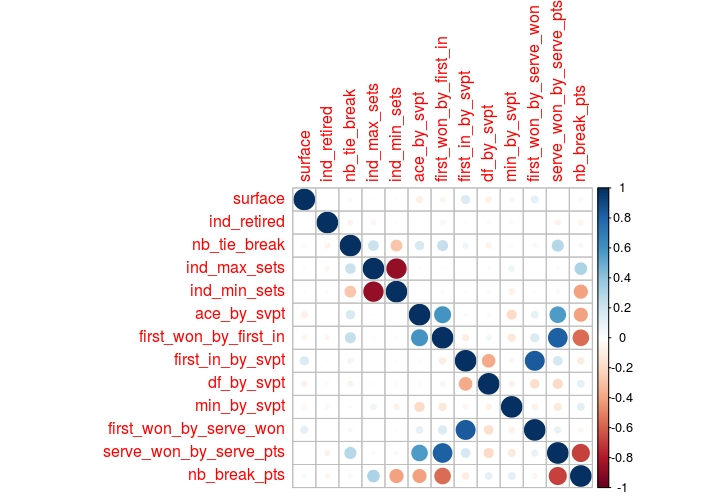
\includegraphics[width=\textwidth]{corrplot}
\end{figure}

On remarque une corrélation positive entre la variable de surface et les variables \texttt{first\_won\_by\_first\_in} et \texttt{first\_won\_by\_serve\_won}. La variable \texttt{ace\_by\_svpt} est corrélée négativement avec la surface. Dans les figures suivantes, on présente le \textit{boxplot} et l'histogramme de \texttt{ace\_by\_svpt} selon la surface.

\begin{figure}[H]
	\caption{\textit{Boxplot} des aces par service en fonction de la surface}
	\label{fig:acebyserve}
	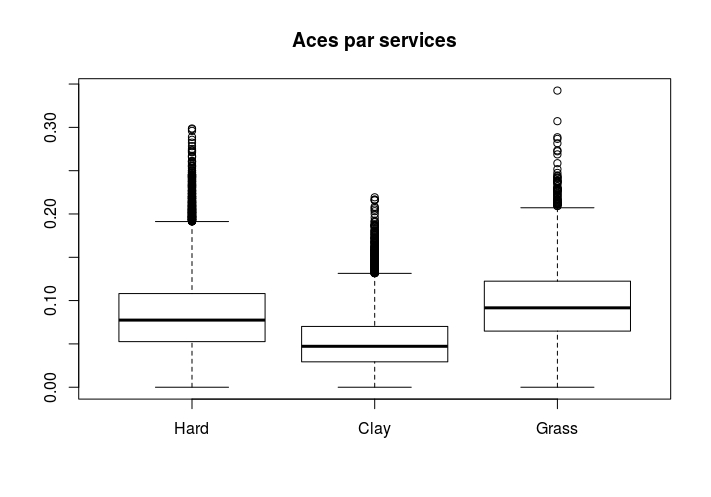
\includegraphics[width=\textwidth]{acevssurface}
\end{figure}

\begin{figure}[H]
	\caption{Histogramme des aces par service en fonction de la surface}
	\label{fig:acebyshist}
	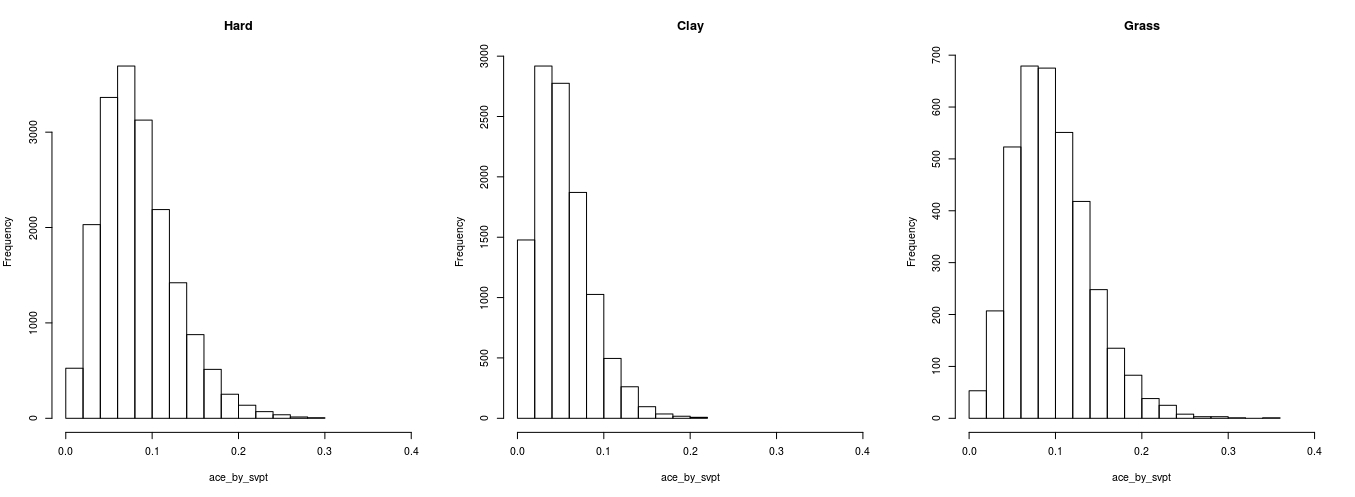
\includegraphics[width=\textwidth]{acebysurfacehist}
\end{figure}

On observe que la distribution de \texttt{ace\_by\_svpt} est de queue moins lourde pour la surface terre battue.\\

Les autres statistiques ne sont pas très intéressantes pour l'analyse. On ne s'attend pas à ce que une seule variable soit plus importante pour les autres pour faire la classification des types de sols.

\subsubsection{Traitement des valeurs manquantes}
Il n'y avait pas réellement de données manquantes dans le jeu de données après avoir fait le premier prétraitement. Ainsi, nous avons utilisé l'analyse des cas complets étant donné qu'un pourcentage très minime des données étaient manquantes (environ 3\%). Nous avons cependant imputé des valeurs de 0 pour les ratios conçus précédemment pour lesquels il y avait une division par zéro.

\subsubsection{Réduction de la dimensionalité}
Tel que mentionné un peu plus tôt, le jeu de données comprend environ une cinquantaine de variables explicatives servant à entraîner un modèle. Ceci peut causer une problème si certaines de ces variables sont non-informatives ou redondantes. Nous avons donc considéré l'approche de faire une analyse en composantes principales (\textit{PCA}) sur le jeu de données et comparer les résultats ceux obtenus sur le jeu de données non réduit. Les projections construitres par l'ACP permet d'obtenir une représentation réduite conservant une grande partie de l'information, produisant les mêmes (ou presque) résultats analytiques. L'ACP a réduit le nombre des variables utilisées à 6, tout en conservant une variance totale supérieure à 80 \%.

\subsection{Classifieurs utilisés}
Les algorithmes d'apprentissage automatique utilisés pour le projet varient en complexité. Nous désirions tester différents niveaux de complexité afin de déterminer si une augmentation de la complexité était justifiée relativement à la qualité des prédictions. Nous avons librement sous-divisé les algorithme utilisés en 3 catégories distinctes. \\ \\
En apprentissage automatique, il y a un compromis à faire entre les connaissances des données et la quantité de données disponibles. Dans le cas où le statisticien connait bien les données, un modèle tres simple, Si le statisticien connait bien les données, il peut utiliser son oppinion pour créer une distribution, comme c'est le cas dans les méthodes paramétriques simples présentés plus loin. En revanche, si le statisticien ne connait pas la distribution des données, il doit utiliser des modèles plus complexes non paramétriques, comme des réseaux de neurones. Dans le milieu de ce compromis, on retrouve des modèles tels que le SVM qui requiert de la connaissance sur le noyau et seulement les hyperparamètres doivent être déterminés.

\subsubsection{Algorithmes simples}
La première catégorie est composée d'algoritmes simples et ne demandant qu'une compréhension générale du modèle afin de les utiliser. Les modèles sont:

\begin{enumerate}
  \item le classifieur de naïf de Bayes, du package e1071 \cite{packagee1071}
  \item le classifieur régression logistique, du package nnet \cite{packagennet} 
  \item l'analyse discriminante linéaire, du package MASS \cite{packageMASS}
  \item l'analyse discriminante quadratique, du package MASS  \cite{packageMASS}
\end{enumerate}

Nous considérons qu'ils sont simples, car ils sont utilisables directement avec une fonction R et ne demandent généralement pas de sélection d'hyperparamètres complexes. De plus, ce sont des modèles paramétriques qui font l'hypothèse qu'il est possible de modéliser les données ** je suis pas clair ici **. 

\subsubsection{Algorithmes intermédiaires}
La deuxième catégorie est composée d'algoritmes un peu plus complexes et demandant un ajustement spécifique de leur hyperparamètres. Ces modèles sont discriminants, c'est à dire qu'ils ne font pas d'hypothèse sur la distribution des données. Les modèles sont:

\begin{enumerate}
  \item le classifieur par arbre, du package rpart \cite{packagerpart}
  \item le classifieur par forêt aléatoire, du package randomForest \cite{packagerandomForest}
  \item le classifieur SVM, du package e1071 \cite{packagee1071}
\end{enumerate}

La méthodologie entourant la sélection des hyperparamètres est présentée dans une section ultérieure.

\subsubsection{Algorithmes complexes}
Finalement, la troisième catégorie est composée d'algoritmes plus complexes et demandant l'utilisation de l'expérience et l'intuition du statisticien. Ce sont des modèles qui n'ont pas été étudiés dans le cours STT-7330 mais qui ont été explorés car ils sont généralement très performants dans les tâches de classification . Les modèles sont:

\begin{enumerate}
  \item les réseaux de neuronnes, du package Keras \cite{packagekeras}
  \item le modèle par ensemble, developpé dans le cadre du projet
\end{enumerate}

L'utilisation et l'architecture de ces modèles seront présentées dans une section ultérieure.

\subsection{Ajustement des hyperparamètres}
L'ajustement des hypersparamètres a été faite par une recherche exhaustive. La technique de recherche par quadrillage (\textit{grid-search}). Afin de ne pas surajuster les modèles lors de cette recherche, nous avons utilisés la validation croisée avec 10 plis.\\ \\ 
La recherche par quadrillage est une technique permettant de trouver les meilleurs hyperparamètres en essayant toutes combinaisons entre les différentes valeurs prédéfinies de chacun de ces hyperparamètres. Comme notre connaissance du jeu de données était plutôt limitée, nous avons décidés de considérer une large gamme de valeurs et de faire une recherche exhaustive pour chacune des combinaison d'hyperparametres possibles.

\subsubsection{Hyperparamètres du modèle par arbre}
Pour le modèle par arbre, les hyperparamètres utilisés sont maxdepth et minsplit. \\\\ 
L'hyperparamètre maxdepth controle la profondeur maximale de l'arbre. La profondeur maximale de l'arbre est en quelque sorte le nombre de divisions pouvant être réalisées dans le jeu de données. En termes du compromis biais-variance, une grande profondeur augmente la variance et réduit le biais. Nous avons considéré les valeurs 1, 3, 5 et 10.\\ \\ 
L'hyperparamètre minsplit controle le nombre de points de données minimum dans un noeud pour qu'il soit divisé. Ainsi plus ce paramètre est grand, plus l'arbre aura des feuille fournies. En termes du compromis biais-variance, un paramètre minsplit élevé donnera à l'arbre une variance faible mais un biais élevé. Nous avons considéré les valeurs de 2, 5, 8, 10, 15 et 20.

\subsubsection{Hyperparamètres du modèle de forêt aléatoire}
Pour le modèle de forêt aléatoire, les hyperparamètres utilisés sont mtry, ntree et nodesize.\\\\ 
L'hyperparamètre mtry contrôle le nombre de variables explicatives sélectionnées aléatoirement lors de la création d'un noeud. En termes du compromis biais-variance, l'augmentation de mtry causera un biais plus petit, mais aura une variance plus grande.  Nous avons considéré les valeurs 4, 8, 12 et 16.\\\\ 
L'hyperparamètre ntree contrôle le nombre d'arbres générés aléatoirement pour créer le classifieur. Il est important d'avoir un nombre suffisamment grand afin de faire baisser la variance et ainsi se rapprocher d'une valeur optimale au niveau du compromis biais-variance. Nous avons considéré les valeurs de 700, 1000 et 2000.\\ \\ 
L'hyperparamètre nodesize contrôle le nombre minimal de données inclus dans le noeud terminal. Par défaut, le paramètre est 1 et cette valeur sur-ajuste les données. Nous avons considéré les valeurs de 3 et 5.

\subsubsection{Hyperparamètres du modèle SVM}
Pour le modèle SVM, les hyperparamètres utilisés sont cost et gamma ($c$ et $\gamma$ dans la notation utilisée dans le cours).\\ \\ 
L'hyperparamètre cost contrôle la fréquence et la sévérité des violations par rapport à la marge. En termes du compromis biais-variance, l'augmentation de cost causera un biais plus grand, mais aura une variance plus petite. Nous avons considéré les valeurs 1, 10, 100 et 1000. L'hyperparamètre gamma est un paramètre de noyau. Nous avons considéré les valeurs 0.001, 0.01, 0.1, 1).\\ \\ 

\subsection{Ajustement des modèles complexes}

\subsubsection{Réseau de neurones}

Finalement, nous avons fait la classification en entraînant un réseau de neurones profond. Les réseaux de neurones sont des modèles très flexibles, mais le choix d'une bonne architecture important. Ces choix sont souvent basés sur beaucoup d'expérience du scientifique des données. Étant donné que le but premier de ce projet n'est pas de construire un réseau de neurones et trouver l'architecture idéale en soi, nous avons choisi une architecture relativement simple. Nous avons donc choisi un réseau à propagation avant avec 2 couches cachées et une couche de sortie à 3 neurones (un pour chacune des catégories possibles) avec du \textit{dropout}. Puisque c'est un problème de classification à multiple classes, nous avons choisi comme mesure de perte la \textit{categorical-crossentropy} et comme métrique à optimiser la précision. La librairie utilisée est celle de \texttt{keras}.\\

Considérant la nature de ce type de méthode, il est important de mentionner le fait que nous n'avons pas structuré les données de la même façon pour ce type de modèle. En effet, celui-ci est mieux adapté pour trouver des interactions dans les variables et il n'est pas nécessaire de travailler en basse dimension. Ainsi, nous n'avons pas construit de variables précises (comme dans la méthode classiques), nous avons plutôt donné en entrée les données brutes au modèle. De plus, les pays d'origine des joueurs sont utilisés (une fois dichotomisés, les pays d'origine des joueurs représentent 156 variables). Un total de 193 variables sont utilisés pour construire le modèle de réseau de neurones.

\subsubsection{Modèles par ensembles}

Les modèles par ensemble sont inspirés du proverbe de la sagesse des foules. Par exemple, si il y a trois classifieurs indépendants qui ont une précision de 0.65 et qu'on utilise un modèle de vote majoritaire, la précision du voteur est 
$$1 - \binom{3}{1}0.65^1\times 0.35^2 + \binom{3}{0}0.65^0\times 0.35^3 = 0.71825.$$
Bien sur, les modèles ne sont pas indépendants car ils utilisent les mêmes données (et parfois des hypothèses similaires). On s'attend quand même à une augmentation de la performance. Ce type de modèle est similaire au modèles AdaBoost et forêt aléatoire qui aggrègent plusieurs apprendants faibles, mais dans notre cas ce sont des apprenants forts.\\

Le vote utilisé est pondéré par la précision du modèle, i.e. un modèle avec une meilleure performance en classification reçoit plus de poids. À partir du jeu de données test, on compare chaque combinaison des voteurs (chaque permutation des 1, 2, \dots, 9 voteurs) et on sélectionne la combinaison qui permet de minimiser l'erreur sur le jeu de données de test.\\

La sortie du modèle est une prédiction basé sur une combinaison de modèles, alors beaucoup d'interprétabilité des résultats est perdu.
